%----------------------------------------
% Write your notes here
%----------------------------------------

\section{Part I - Classification Continued}
\subsection{Naive Bayes}

We saw that Naive Bayes fundementally was ``Naive'' due in part by the naive assumption that each feature was independent from each other conditioned on their class.  

We took a look at the classic spam filtering problem.  We have an email with D words so each email can be represented by a vector $\mathbf{x} \in \mathbb{R}^D$, where the ith component of $\mathbf{x}$, is denoted as $x_i$, represents the ith word in the email.  Our goal is to classify this email as spam or ham (not spam).  Usually D is on the scale of 500k to 100k.  

\begin{itemize}
\item 
 $\vec{\mathbf{x}} = ( \text{I am a Nigerian prince and I need your help} ) $
\end{itemize}

Using Bayes Rule, we have the following: 

\begin{equation}
P(A | B ) P(B) = P(A \cap B) = P(B | A ) P(A) = ~~ \Rightarrow ~~ P(c | \mathbf{x}) = P(\mathbf{x} | c ) \frac{P(c)}{P(\mathbf{x})}
\end{equation}

Here $c$ denotes a certain class.  In this case, $c \in \{ \text{spam}, \text{not spam} \}$.   

\indent 

The naive part of Naive Bayes says: 
$$
P(\mathbf{x} | c ) = \prod\lines_{i=1}^D P(x_i | c) 
$$

Consequrently (1) becomes, 

\begin{equation}
P(c | \mathbf{x}) = \prod\lines_{i=1}^D P(x_i | c)  \frac{P(c)}{P(\mathbf{x})}
\end{equation}

We model each term in the series of products to be a coin flip.  In other words, $P(x_j | c)$ will represent the distribution of a Bernoulli random variable $X_j$, which we will have an associated parameter $\theta_{jc}$. $\theta_{jc}$ represents the probablity that the jth word appears under class $c$. 

\begin{equation}
P(x_j | c ) = \theta_{jc}^{x_j} (1 - \theta_{jc}^{1 - x_j})
\end{equation}

With this in mind and denoting $P(c) = \theta_c$, we plug this back into (2) and take the log of the Likelihood to get: 

$$
\log(p(c | \mathbf{x})) = \log \left ( \prod\lines_{i=j}^D \theta_{jc}^{x_j} (1 - \theta_{jc}^{1 - x_j})  \frac{P(c)}{P(\mathbf{x})} \right) = \log \left ( \prod\lines_{i=j}^D \theta_{jc}^{x_j} (1 - \theta_{jc}^{1 - x_j} \right) + \log \left( \frac{\theta_c}{P(\mathbf{x})} \right)
$$

$$
\Rightarrow \sum\lines_{j=1}^D \log[ \theta_{jc}^{x_j} (1 - \theta_{jc})^{1-x_j}] + \log \frac{\theta_c}{P(\mathbf{x})} = \sum\lines_{j=1}^D x_j \log \theta_{jc} + \sum\lines_{j=1}^D (1-x_j) \log(1 - \theta_{jc}) + \log \frac{\theta_c}{P(\mathbf{x})}
$$

$$
\sum\lines_{j=1}^D x_j \log \theta_{jc} + \sum\lines_{j=1}^D \log(1 - \theta_{jc}) - \sum\lines_{j=1}^D x_j \log(1 - \theta_{jc}) + \log \frac{\theta_c}{P(\mathbf{x})}
$$

\begin{equation}
\log(p(c | \mathbf{x})) = \sum\lines_{j=1}^D x_j \log \frac{ \theta_{jc}}{1 - \theta_{jc}} + \sum\lines_{j=1}^D \log(1 - \theta_{jc}) +  \log \frac{\theta_c}{P(\mathbf{x})} 
\end{equation}

To find $P(\mathbf{x})$, we can condition $\mathbf{x}$ on the number of classes and multiply by the respective probabilities of being in that class.  

$$
P(\mathbf{x}) = \sum\lines_c P(\mathbf{x}, c) = \sum\lines_c P(\mathbf{x} | c) P(c)
$$

Restricting ourselves to the 2-class example problem at hand, $c$ can only take values 0 (not spam) or 1 (spam).  Taking the difference in probability between an email being in class 1 and that same email being in class 0, we have: 
\begin{equation}
P( c = 1 | \mathbf{x}) - P( c = 0 | \mathbf{x}) ~~ \Rightarrow ~~ 
\log \frac{  P( c = 1 | \mathbf{x})}{P( c = 0 | \mathbf{x})}
\end{equation}

Using equation (4) to calculate $P(c = 1 | \mathbf{x}) $ and $P(c = 0 | \mathbf{x}) $ :

\begin{equation}
\log P(c = 1 | \mathbf{x}) = \sum\lines_{j=1}^D x_j \log \frac{ \theta_{j1}}{1 - \theta_{j1}} + \sum\lines_{j=1}^D \log(1 - \theta_{j1}) +  \log \frac{\theta_1}{P(\mathbf{x})} 
\end{equation}

\begin{equation}
\log P(c = 0 | \mathbf{x}) = \sum\lines_{j=1}^D x_j \log \frac{ \theta_{j0}}{1 - \theta_{j0}} + \sum\lines_{j=1}^D \log(1 - \theta_{j0}) +  \log \frac{\theta_0}{P(\mathbf{x})} 
\end{equation}

Taking the difference between (6) and (7) is equivalent to (5). 

$$
\sum\lines_{j=1}^D x_j \log \frac{ \theta_{j1}}{1 - \theta_{j1}} + 
\sum\lines_{j=1}^D \log(1 - \theta_{j1}) +  \log \frac{\theta_1}{P(\mathbf{x})} - \left( \sum\lines_{j=1}^D x_j \log \frac{ \theta_{j0}}{1 - \theta_{j0}} + \sum\lines_{j=1}^D \log(1 - \theta_{j0}) +  \log \frac{\theta_0}{P(\mathbf{x})} \right)
$$

$$
\Rightarrow \log \frac{  P( c = 1 | \mathbf{x})}{P( c = 0 | \mathbf{x})} = 
\sum\lines_{j=1}^D x_j \log \frac{ \theta_{j1} ( 1 - \theta_{j0}) }{ \theta_{j0}  (1 - \theta_{j1} ) } + 
\sum\lines_{j=1}^D \log \frac{ 1 - \theta_{j1} }{ 1 - \theta_{j0}  } +
 \log \frac{\theta_1}{\theta_0}
$$

Defining $ \log \frac{ \theta_{j1} ( 1 - \theta_{j0}) }{ \theta_{j0}  (1 - \theta_{j1} ) } = w_j $ where $\mathbf{w} = ( w_1, \dots, w_D) \in \mathbb{R}^D$, then we describe the difference between these log probabilities as:  

\begin{equation}
\log \frac{  P( c = 1 | \mathbf{x})}{P( c = 0 | \mathbf{x})} = 
\mathbf{x} \cdot \mathbf{w} + w_0
\end{equation}

As a side note, $w_0 = log \frac{\theta_1}{\theta_)}$ and therefore this term can be computed without knowing x. 

How this relate to classification?  Intuitively, we want to classify a vector $\mathbf{x}$ to be in a certain class if it has the highest probability of belong in that class.  In the 2-class case, we classify $\mathbf{x}$ to be in class 1 only if $P( c = 1| \mathbf{x}) > P( c = 0 | \mathbf{x}) $  or we classify it to be in class 0 only if $P( c = 1| \mathbf{x}) < P( c = 0 | \mathbf{x}) $. Because log is a monotonically increasing function then all of these results hold if we log both sides.  


$$
\log \frac{  P( c = 1 | \mathbf{x})}{P( c = 0 | \mathbf{x})} = \log P( c = 1 | \mathbf{x}) - \log P( c = 0 | \mathbf{x})
$$

Therefore, if $\mathbf{x}$ is in class 1, we have $ \log P( c = 1| \mathbf{x}) > \log P( c = 0 | \mathbf{x})  ~~ \Rightarrow ~~ \log P( c = 1| \mathbf{x}) - \log P( c = 0 | \mathbf{x}) > 0 $.  

In other words, if $\log \frac{  P( c = 1 | \mathbf{x})}{P( c = 0 | \mathbf{x})} = 
\mathbf{x} \cdot \mathbf{w} + w_0 > 0$, we classify $\mathbf{x}$ to be in 1, otherwise if it is $< 0$, we classify it as class 0.  


All this is left is finding the appropriate parameters $\theta_{jc}$ for the jth word that belongs in a certain class.  The best value is determined by maximizing the likelihood with respect to the parameters $\theta$. 

In class, the way we approached this seemingly complex problem is by simply loooking at the following problem:   Imagine tossing a coin $N$ times that lands hands with probability $\theta$.  Further imagine that of these $N$ tosses, we observed heads $n$ times.  Then:

$$
P( n \text{ heads} | \theta ) = C \theta^{n} (1 - \theta)^{N -n} \text{ Where C is some aribtrary constant. }
$$


$$
\ell = \log P( n \text{ heads} | \theta ) = \log(C) +  n \log(\theta) + (N - n) \log(1 - \theta)
$$

$$
\frac{d \ell}{d \theta} = \frac{n}{\theta} - \frac{N-n}{1-\theta} = 0 ~~ \Rightarrow ~~ n - n\theta = \theta N -\theta n ~~ \Rightarrow ~ \theta = \frac{n}{N} = \frac{ \text{ \# head occurs } }{\text{ total tosses }}
$$

Then, the best estimators in our model are: 
\begin{equation}
\theta_{j1} = \frac{n_{j1} }{n_1} = \frac{\# \text{ spam docs with word j }} {\# \text{ spam documents}}
\end{equation}

\begin{equation}
\theta_{j0} = \frac{n_{j0} }{n_0} = \frac{\# \text{ non-spam docs with word j }}{\# \text{ non-spam documents}}
\end{equation}

\begin{equation}
\theta_1 = \frac{n_1}{N} = \frac{\# \text{ spam documents} }{\# \text{ total docs}} ~~~~ \theta_0 = \frac{n_0}{N} = \frac{\# \text{ non-spam documents} }{\# \text{ total docs}} 
\end{equation}

\subsubsection {Runtime Complexity}
The run time complexity of running Naive Bayes with $N$ documents and $K$, the number of words in our vocabulary, is $\mathcal{O}(KN)$ if we're not being clever. However, to improve efficeincy all we have to do is run through the data set only once and keep track of words that appear.  Therefore, our run time is $\mathcal{O}(\bar{k} N)$, where $\bar{k}$ is the average number of words in a document. This run time is the time complexity.  It requires us to run through all the documents, where in each run we append the document to a dictionary and then create a new dictionary associated with this document with all the counts of the words.  

The Naive Bayes model can be updated continually as it sees more and more data because the parameters $\theta$ would simply get incremented in the appropriate fashion.

\subsection{Logistic Regression}

Wht if we just start with a predictor of the same form that we derived in Naive Bayes with some unknown weights?  What we would find in solving for the probability of being in some class 1.  (i.e p is the probability something is classified as class 1), we would get:


\begin{equation}
\log \frac{p}{ 1 - p} = \mathbf{w} \cdot \mathbf{x} ~~~~ \text{ where the intercept has been adding implcitly into the vector w}
\end{equation}

\pagebreak 
Solving for p leads us with the following sigmoid function, which looks like the graph below in 2-dimensions:

\begin{equation}
p = \frac{1}{ 1 + e^{- \mathbf{w} \cdot \mathbf{x}}}
\end{equation}

\begin{figure}[ht]
  \begin{center}
    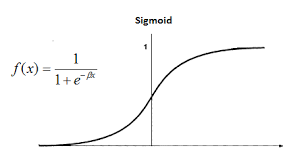
\includegraphics[width=0.5\textwidth]{figures/sigmoid.png}
    \caption{
      A graph of a sigmoid function in 2 dimensions. }
    \label{Figure 1}
  \end{center}
\end{figure}

In this case, as $p \to 1$, the higher the probability we have that this vector is a part of class 1.  

Like in other Machine Learning models, we need to find the optimal parameters.  We turn to maximum likelihood and defining a form of loss that we hope to minimize.  Note, each vector $\mathbf{x}_i$ has an associated class label $y_i$ and $p_i = P(\mathbf{x}_i | \mathbf{w})$.  

Our likelihood function is:  

$$
L = \prod_i p_i^{y_i} (1 - p_i)^{ 1- y_i}
$$

Our loss function is therefore: 

\begin{equation}
\mathcal{L} = - \log P(\text{ data } | \mathbf{w}) = - \sum_i y_i \log p_i + (1 - y_i) \log( 1 - p_i)
\end{equation}

This simplifies to:

$$
\Rightarrow  - \sum_i y_i \log p_i + \log ( 1 - p_i ) - y_i \log(1 - p_i) = - \sum_i y_i \log \frac{p_i}{ 1 - p_i} + \log ( 1 - p_i) 
$$

$$
\mathcal{L}  = - \sum_i y_i \mathbf{w} \cdot \mathbf{x}_i - \log ( 1 + e^{\mathbf{w} \cdot \mathbf{x}})
$$

We need to find the optimal $\mathbf{w}$, so we'll turn to some basic calculus: 

$$
\frac{ \partial \mathcal{L}}{\partial w_k} = - \sum_i y_i x_{ik} - \frac{e^{\mathbf{w} \cdot \mathbf{x}_i } x_{ik}}{1 + e^{\mathbf{w} \cdot \mathbf{x}_i }}  = 0
~~~ w_k \text{ is the kth component of the vector} \mathbf{w}
$$

For each component of the vector w, we have a transcendental equation which has no closed form solution.  

We turn to gradient descent, and have the following update equations: 

$$
\mathbf{w} \leftarrow \mathbf{w} - \eta \frac{ \partial \mathcal{L}}{\partial \mathbf{w}}  ~~ \Rightarrow ~~ 
\mathbf{w} \leftarrow \mathbf{w} + \eta \mathbf{x}^T( y - \text{prediction})
$$

In Naive Byaes we estimate all the w's as independent from each other but in logisitic regression the w's are dependent.  
Logistic Regression won't have an over confidence problem like Naive Bayes has.  

\pagebreak
\subsubsection{Regularized Logistic Regresssion}

If we want to prevent overfitting and prevent the components in our vector of parameters $w$ from getting to big, we can constrain our loss function by doing the following: 

\begin{equation}
\mathcal{L} = - \sum_i y_i \log p_i + (1 - y_i) \log( 1 - p_i) + \frac{1}{2} \lambda^2
\end{equation}

Again finding the optimal value of this expression gives us the following:  

$$
\frac{ \partial \mathcal{L}}{\partial w_k} = - \sum_i (y_i - p_i)y_{ik} +\lambda w_{k} = 0
$$

We get the following new update equations in our gradent descent algorithm: 

$$
w_k \leftarrow w_k - \eta \frac{\partial x}{\partial w_k} \Rightarrow
w_k \leftarrow w_k + \eta \sum_i (y_i - p_i)x_{ik} - \lambda w_k
$$

\begin{equation}
w_k \leftarrow (1 - \eta \lambda) w_k + \eta \sum_i (y_i - p_i)x_{ik}
\end{equation}

We are essentially shrinknig our weight before we move against the gradient.  


\section{ Model Evaluation}

Last time we saw the following definitions of accuracy and calibration: 

\textbf{Accuracy: } Fraction of times you predict the correct label.

\textbf{Calibration: } how often does a event with predicted probability $p$ occur?  




























